% Options for packages loaded elsewhere
\PassOptionsToPackage{unicode}{hyperref}
\PassOptionsToPackage{hyphens}{url}
%
\documentclass[
  10pt,
  letterpaper,
  DIV=11,
  numbers=noendperiod,
  twoside]{scrartcl}

\usepackage{amsmath,amssymb}
\usepackage{setspace}
\usepackage{iftex}
\ifPDFTeX
  \usepackage[T1]{fontenc}
  \usepackage[utf8]{inputenc}
  \usepackage{textcomp} % provide euro and other symbols
\else % if luatex or xetex
  \usepackage{unicode-math}
  \defaultfontfeatures{Scale=MatchLowercase}
  \defaultfontfeatures[\rmfamily]{Ligatures=TeX,Scale=1}
\fi
\usepackage{lmodern}
\ifPDFTeX\else  
    % xetex/luatex font selection
  \setmainfont[ItalicFont=EB Garamond Italic,BoldFont=EB Garamond
Bold]{EB Garamond Math}
  \setsansfont[]{Europa-Bold}
  \setmathfont[]{Garamond-Math}
\fi
% Use upquote if available, for straight quotes in verbatim environments
\IfFileExists{upquote.sty}{\usepackage{upquote}}{}
\IfFileExists{microtype.sty}{% use microtype if available
  \usepackage[]{microtype}
  \UseMicrotypeSet[protrusion]{basicmath} % disable protrusion for tt fonts
}{}
\usepackage{xcolor}
\usepackage[left=1in, right=1in, top=0.8in, bottom=0.8in,
paperheight=9.5in, paperwidth=6.5in, includemp=TRUE, marginparwidth=0in,
marginparsep=0in]{geometry}
\setlength{\emergencystretch}{3em} % prevent overfull lines
\setcounter{secnumdepth}{3}
% Make \paragraph and \subparagraph free-standing
\ifx\paragraph\undefined\else
  \let\oldparagraph\paragraph
  \renewcommand{\paragraph}[1]{\oldparagraph{#1}\mbox{}}
\fi
\ifx\subparagraph\undefined\else
  \let\oldsubparagraph\subparagraph
  \renewcommand{\subparagraph}[1]{\oldsubparagraph{#1}\mbox{}}
\fi


\providecommand{\tightlist}{%
  \setlength{\itemsep}{0pt}\setlength{\parskip}{0pt}}\usepackage{longtable,booktabs,array}
\usepackage{calc} % for calculating minipage widths
% Correct order of tables after \paragraph or \subparagraph
\usepackage{etoolbox}
\makeatletter
\patchcmd\longtable{\par}{\if@noskipsec\mbox{}\fi\par}{}{}
\makeatother
% Allow footnotes in longtable head/foot
\IfFileExists{footnotehyper.sty}{\usepackage{footnotehyper}}{\usepackage{footnote}}
\makesavenoteenv{longtable}
\usepackage{graphicx}
\makeatletter
\def\maxwidth{\ifdim\Gin@nat@width>\linewidth\linewidth\else\Gin@nat@width\fi}
\def\maxheight{\ifdim\Gin@nat@height>\textheight\textheight\else\Gin@nat@height\fi}
\makeatother
% Scale images if necessary, so that they will not overflow the page
% margins by default, and it is still possible to overwrite the defaults
% using explicit options in \includegraphics[width, height, ...]{}
\setkeys{Gin}{width=\maxwidth,height=\maxheight,keepaspectratio}
% Set default figure placement to htbp
\makeatletter
\def\fps@figure{htbp}
\makeatother
% definitions for citeproc citations
\NewDocumentCommand\citeproctext{}{}
\NewDocumentCommand\citeproc{mm}{%
  \begingroup\def\citeproctext{#2}\cite{#1}\endgroup}
\makeatletter
 % allow citations to break across lines
 \let\@cite@ofmt\@firstofone
 % avoid brackets around text for \cite:
 \def\@biblabel#1{}
 \def\@cite#1#2{{#1\if@tempswa , #2\fi}}
\makeatother
\newlength{\cslhangindent}
\setlength{\cslhangindent}{1.5em}
\newlength{\csllabelwidth}
\setlength{\csllabelwidth}{3em}
\newenvironment{CSLReferences}[2] % #1 hanging-indent, #2 entry-spacing
 {\begin{list}{}{%
  \setlength{\itemindent}{0pt}
  \setlength{\leftmargin}{0pt}
  \setlength{\parsep}{0pt}
  % turn on hanging indent if param 1 is 1
  \ifodd #1
   \setlength{\leftmargin}{\cslhangindent}
   \setlength{\itemindent}{-1\cslhangindent}
  \fi
  % set entry spacing
  \setlength{\itemsep}{#2\baselineskip}}}
 {\end{list}}
\usepackage{calc}
\newcommand{\CSLBlock}[1]{\hfill\break\parbox[t]{\linewidth}{\strut\ignorespaces#1\strut}}
\newcommand{\CSLLeftMargin}[1]{\parbox[t]{\csllabelwidth}{\strut#1\strut}}
\newcommand{\CSLRightInline}[1]{\parbox[t]{\linewidth - \csllabelwidth}{\strut#1\strut}}
\newcommand{\CSLIndent}[1]{\hspace{\cslhangindent}#1}

\setlength\heavyrulewidth{0ex}
\setlength\lightrulewidth{0ex}
\usepackage[automark]{scrlayer-scrpage}
\clearpairofpagestyles
\cehead{
  Brian Weatherson
  }
\cohead{
  Four Problems in Decision Theory
  }
\ohead{\bfseries \pagemark}
\cfoot{}
\makeatletter
\newcommand*\NoIndentAfterEnv[1]{%
  \AfterEndEnvironment{#1}{\par\@afterindentfalse\@afterheading}}
\makeatother
\NoIndentAfterEnv{itemize}
\NoIndentAfterEnv{enumerate}
\NoIndentAfterEnv{description}
\NoIndentAfterEnv{quote}
\NoIndentAfterEnv{equation}
\NoIndentAfterEnv{longtable}
\NoIndentAfterEnv{abstract}
\renewenvironment{abstract}
 {\vspace{-1.25cm}
 \quotation\small\noindent\rule{\linewidth}{.5pt}\par\smallskip
 \noindent }
 {\par\noindent\rule{\linewidth}{.5pt}\endquotation}
\KOMAoption{captions}{tableheading}
\makeatletter
\@ifpackageloaded{caption}{}{\usepackage{caption}}
\AtBeginDocument{%
\ifdefined\contentsname
  \renewcommand*\contentsname{Table of contents}
\else
  \newcommand\contentsname{Table of contents}
\fi
\ifdefined\listfigurename
  \renewcommand*\listfigurename{List of Figures}
\else
  \newcommand\listfigurename{List of Figures}
\fi
\ifdefined\listtablename
  \renewcommand*\listtablename{List of Tables}
\else
  \newcommand\listtablename{List of Tables}
\fi
\ifdefined\figurename
  \renewcommand*\figurename{Figure}
\else
  \newcommand\figurename{Figure}
\fi
\ifdefined\tablename
  \renewcommand*\tablename{Table}
\else
  \newcommand\tablename{Table}
\fi
}
\@ifpackageloaded{float}{}{\usepackage{float}}
\floatstyle{ruled}
\@ifundefined{c@chapter}{\newfloat{codelisting}{h}{lop}}{\newfloat{codelisting}{h}{lop}[chapter]}
\floatname{codelisting}{Listing}
\newcommand*\listoflistings{\listof{codelisting}{List of Listings}}
\makeatother
\makeatletter
\makeatother
\makeatletter
\@ifpackageloaded{caption}{}{\usepackage{caption}}
\@ifpackageloaded{subcaption}{}{\usepackage{subcaption}}
\makeatother
\ifLuaTeX
  \usepackage{selnolig}  % disable illegal ligatures
\fi
\IfFileExists{bookmark.sty}{\usepackage{bookmark}}{\usepackage{hyperref}}
\IfFileExists{xurl.sty}{\usepackage{xurl}}{} % add URL line breaks if available
\urlstyle{same} % disable monospaced font for URLs
\hypersetup{
  pdftitle={Four Problems in Decision Theory},
  pdfauthor={Brian Weatherson},
  hidelinks,
  pdfcreator={LaTeX via pandoc}}

\title{Four Problems in Decision Theory}
\author{Brian Weatherson}
\date{2024}

\begin{document}
\maketitle
\begin{abstract}
In recent years the literature on decision theory has become disjointed.
There isn't as much discussion as there should be on how different
problems impact one another. This paper aims to bring together work on
problems involving demons, problems about attitudes to risk, problems
about incomplete preferences, and problems about dynamic choice. In the
first three of these cases, I end up defending a pre-existing view. I
defend a ratificationist approach to problems with demons, the orthodox
expected utility approach to risk, and the permissibility of incomplete
preferences. These views are familiar, but seeing how they are related
to a common strengthens the case for each of them. The most novel part
of the view is the theory of dynamic choice that I offer: a sequence of
choices is rational only if both the so-called `resolute' and
`sophisticated' theories of dynamic choice would permit it. This theory
would be implausible if paired with many rival solutions to the first
three problems, but fits nicely with the view I'll develop through the
paper.
\end{abstract}

\setstretch{1.1}
Contemporary decision theory has become disjointed. There is less
overlap than there should be in work on adjacent problems. This paper
aims to undo some of that, by showing that four problems that have
largely been worked on in isolation cast useful light on each other. In
particular, I'll argue that we can go a long way towards solving all
four problems by working through the consequences of a plausible
principle that I'll call the Single Choice Principle.

The Single Choice Principle (hereafter, SCP) relates theories of static
choice and dynamic choice. In particular, it says that for a narrow
class of games, it doesn't matter whether you think of the game as
involving a static, strategic choice, or a dynamic choice that is made
during a game. One way into the principle is to think about an oddity in
the way Newcomb's Problem is normally introduced.

\section{Newcomb's Problem}\label{newcombs-problem}

\subsection{Standard Version}\label{standard-version}

In the standard vignette that goes with Newcomb's Problem, it is a
dynamic game. The demon makes a \emph{prediction}, and then the human
(hereafter, Chooser) makes a choice. Chooser doesn't know what Demon
did, but they do know that Demon has acted. So the natural presentation
of Newcomb's Problem is in a tree like
Figure~\ref{fig-standard-newcomb}.\footnote{I'll assume \$1,000 is worth
  1 util. I think this assumption of constant marginal utility is close
  to incoherent, and it will get relaxed later, but it's harmless for
  now.}

\subsection{Tree}

\begin{figure}

\centering{

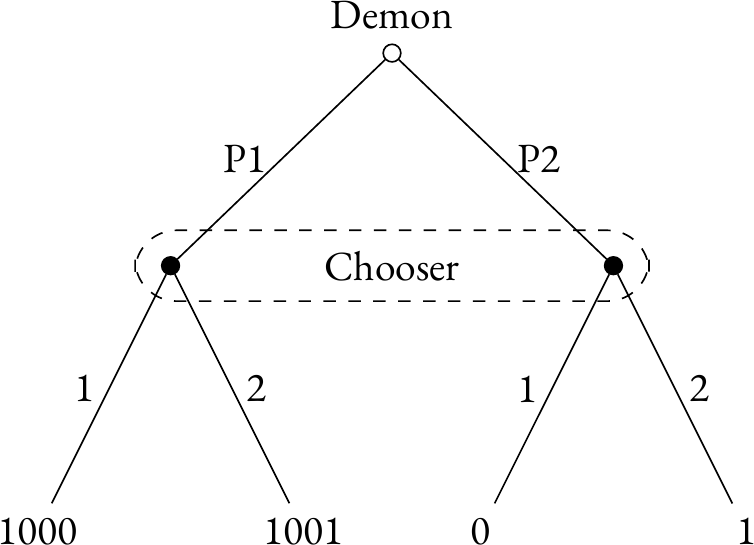
\includegraphics{four-problems-march-25-2024_files/figure-pdf/fig-standard-newcomb-1.png}

}

\caption{\label{fig-standard-newcomb}Newcomb's Problem.}

\end{figure}%

\subsection{Table}

\begin{longtable}[]{@{}ccc@{}}
\caption{Newcomb's Problem}\label{tbl-standard-newcomb}\tabularnewline
\toprule\noalign{}
& P1 & P2 \\
\midrule\noalign{}
\endfirsthead
\toprule\noalign{}
& P1 & P2 \\
\midrule\noalign{}
\endhead
\bottomrule\noalign{}
\endlastfoot
1 & 1000 & 0 \\
2 & 1001 & 1 \\
\end{longtable}

I'll go over the details of how to read diagrams like
Figure~\ref{fig-standard-newcomb} in {[}insert cross-ref here!{]}. All
you need to know for now is that the game starts at the open node, here
at the top, and it moves along by the agent (Demon or Chooser) making
choices. The dotted lines around the two nodes where Chooser acts mean
that those two nodes are in the same \textbf{information set}. That is,
when Chooser is at either one of those nodes, the strongest thing
Chooser knows is that they are somewhere or other in the set.\footnote{This
  formalism only really makes sense if we presuppose the right epistemic
  logic is S5, and there are good reasons to not make that assumption in
  general (\citeproc{ref-Humberstone2016}{Humberstone 2016, 380--402}).
  For this paper we'll treat it as a simplifying assumption that really
  should be relaxed in subsequent work.} So this tree represents the
standard vignette for Newcomb's Problem. Demon makes a prediction - I'm
in general using PX for Demon predicting X - and Chooser knows that the
prediction has been made, and that either P1 or P2 happened, but chooses
without knowing which it is. Then the game is resolved.

What Table~\ref{tbl-standard-newcomb} shows is a subtly different story.
In Table~\ref{tbl-standard-newcomb}, each player chooses a
\emph{strategy}. A strategy for a player in a tree like
Figure~\ref{fig-standard-newcomb} is a decision about what to do at each
node in the tree where that player has to move.\footnote{In game theory,
  it is usually specified that strategies include decisions about what
  to do at nodes that are ruled out by earlier moves in that very
  strategy. In theory I'm assuming this whenever I talk about
  strategies; in practice it doesn't matter for any application in this
  paper.} So what Table~\ref{tbl-standard-newcomb} represents is a
situation where each player chooses a strategy simultaneously, and that
determines a result for the game. It differs from
Figure~\ref{fig-standard-newcomb} in part in that it's symmetric; there
is no hint that Demon moves first.

There is a lot of disagreement about Newcomb's Problem, but here is one
point of universal agreement: Figure~\ref{fig-standard-newcomb} and
Table~\ref{tbl-standard-newcomb} have the same solutions. It would be
incoherent to prefer taking 1 box in one of these puzzles and 2 boxes in
the other, or to say that both options were choice-worthy in one puzzle
but not the other. They may not represent exactly the same problem, they
don't pose exactly the same question to Chooser, but they should get the
same answer (or answers).

I'm going to agree with the unanimous verdict on this point, but I'll
start dissenting very soon. And one way into my dissent is to ask, why
should Figure~\ref{fig-standard-newcomb} and
Table~\ref{tbl-standard-newcomb} get the same answer? What principle is
someone who gives different answers to the two questions violating? I
have a suggestion for what principle that might be, the SCP, but to make
that suggestion plausible we need a couple more examples.

\subsection{Variant 1: Coin-then-Demon}\label{variant-1-coin-then-demon}

Consider a variant on Newcomb's Problem I'll call Coin-Then-Demon. In
this game a fair coin will be flipped and shown to Demon and Chooser. If
it lands Heads, Chooser will get \$5,000 and the game ends. Otherwise,
they play standard Newcomb Problem. Figure~\ref{fig-coin-then-demon}
shows the game tree for this game, with Nature moving first, and the
probabilities of Nature's moves shown. And
Table~\ref{tbl-coin-then-demon} shows the strategy table for it, with
the payouts shown in expected value.\footnote{I will drop the assumption
  that Chooser maximises expected value in Section~\ref{sec-buchak}, but
  it's a harmless assumption for now.}

\subsection{Tree}

\begin{figure}

\centering{

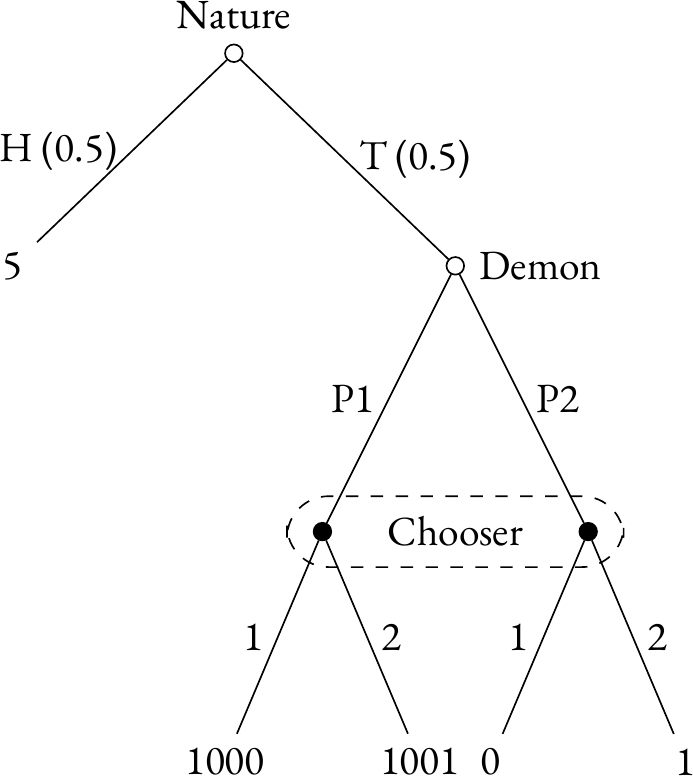
\includegraphics{four-problems-march-25-2024_files/figure-pdf/fig-coin-then-demon-1.png}

}

\caption{\label{fig-coin-then-demon}Coin-then-Demon}

\end{figure}%

\subsection{Table}

\begin{longtable}[]{@{}ccc@{}}
\caption{Coin-then-Demon}\label{tbl-coin-then-demon}\tabularnewline
\toprule\noalign{}
& P1 & P2 \\
\midrule\noalign{}
\endfirsthead
\toprule\noalign{}
& P1 & P2 \\
\midrule\noalign{}
\endhead
\bottomrule\noalign{}
\endlastfoot
1 & 502.5 & 2.5 \\
2 & 503 & 3 \\
\end{longtable}

I have two hypotheses about
Figure~\ref{fig-coin-then-demon}/Table~\ref{tbl-coin-then-demon}; one of
which I think everyone will agree with, and one that might be more
controversial. The less controversial hypothesis is that in this game,
as in standard Newcomb's Problem, it doesn't matter whether Chooser is
playing the dynamic game (i.e., Figure~\ref{fig-coin-then-demon}) or the
strategic game (i.e., Table~\ref{tbl-coin-then-demon}). Whichever
options are choice-worthy in one are choice-worthy in the other. The
more controversial hypothesis is that the reason these two games are
rationally equivalent is exactly the same as the reason that the two
forms of Newcomb Problem I presented should get the same answer.

\subsection{Variant 2: Demon-then-Coin}\label{variant-2-demon-then-coin}

One more example and we're basically done. In the game I'll call
Demon-Then-Coin, the coin is only flipped if Demon predicts Chooser
takes one box. If the coin lands heads, Chooser gets \$5,000, and the
game ends. If either Demon predicts 2 boxes, or the coin lands tails,
Chooser makes a selection, knowing that one or other of these disjuncts
obtained. Then the game ends. The tree for this game is
Figure~\ref{fig-demon-then-coin}, and the strategy table is
Table~\ref{tbl-demon-then-coin}.

\subsection{Tree}

\begin{figure}

\centering{

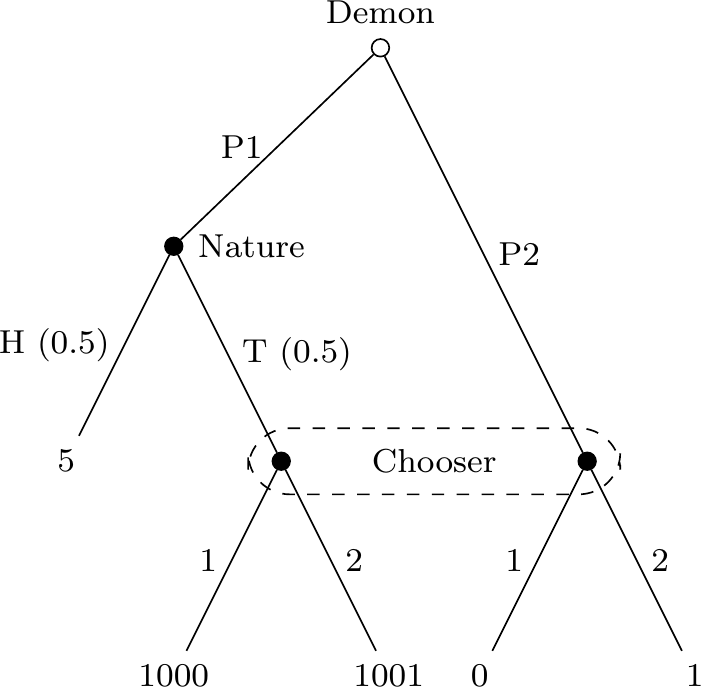
\includegraphics{four-problems-march-25-2024_files/figure-pdf/fig-demon-then-coin-1.png}

}

\caption{\label{fig-demon-then-coin}Demon-then-Coin}

\end{figure}%

\subsection{Table}

\begin{longtable}[]{@{}ccc@{}}
\caption{Demon-then-Coin}\label{tbl-demon-then-coin}\tabularnewline
\toprule\noalign{}
& P1 & P2 \\
\midrule\noalign{}
\endfirsthead
\toprule\noalign{}
& P1 & P2 \\
\midrule\noalign{}
\endhead
\bottomrule\noalign{}
\endlastfoot
1 & 502.5 & 0 \\
2 & 503 & 1 \\
\end{longtable}

If Chooser was planning on picking 1 box, they have a little evidence
against the accuracy of Demon's predictions. If in the other games they
thought the probability that Demon mispredicted was \emph{e}, in this
case they should (if they plan to choose 1 box) have a probability of
error of roughly 2\emph{e}. But if \emph{e} was small enough to start
with, and I'll assume throughout that Demon's error likelihood is
arbitrarily small, this shouldn't make a difference.

Again, I'm going to argue that the dynamic game,
Figure~\ref{fig-demon-then-coin}, and the strategic game,
Table~\ref{tbl-demon-then-coin}, should get the same solutions. Indeed,
they should get the same solutions for the same reason the previous two
pairs of

\subsection{Single Choice Principle}\label{single-choice-principle}

Quote the definition

\section{Defending the SCP}\label{sec-scp-defence}

\subsection{Ramsey Test}\label{ramsey-test}

\subsection{Unifying the Examples}\label{unifying-the-examples}

\subsection{Intuitions about Change}\label{intuitions-about-change}

\subsection{No Reward}\label{no-reward}

Stress that asymmetry cases are most plausible when the strategy
suggests that you'll actually make the dodgy choice with very low
probability.

\subsection{Sure Thing}\label{sure-thing}

\section{The Four Problems}\label{the-four-problems}

\subsection{Demonic Problems}\label{demonic-problems}

Stress the Stag Hunt and coordination games

\subsection{Buchak}\label{sec-buchak}

\subsection{Incomplete Preferences}\label{incomplete-preferences}

\subsection{Dynamic Choice}\label{dynamic-choice}

\section{Ratificationism}\label{ratificationism}

Go over the 4,3,2 game

Show that CDT, EDT, and most other views violate SCP

\section{Expected Value}\label{expected-value}

Buchak stuff, goes really fast

\section{Incomplete Preferences}\label{incomplete-preferences-1}

Again, the 4,3,2 shows this really quickly, I think this is already
written

\section{Dynamic Choice}\label{dynamic-choice-1}

This takes much more time.

\section{Conclusion}\label{conclusion}

Paragraph about how this connects to game theory

Summary of what we've shown.

\phantomsection\label{refs}
\begin{CSLReferences}{1}{0}
\bibitem[\citeproctext]{ref-Humberstone2016}
Humberstone, Lloyd. 2016. \emph{Philsophical Applications of Modal
Logic}. Milton Keynes: College Publications.

\end{CSLReferences}



\noindent Unpublished. Posted online in 2024.

\end{document}
